\documentclass{standalone}
\usepackage{tikz}
\usepackage{ctex,siunitx}
\setCJKmainfont{Noto Serif CJK SC}
\usepackage{tkz-euclide}
\usepackage{amsmath}
\usetikzlibrary{patterns, calc,3d}
\usetikzlibrary {decorations.pathmorphing,decorations.pathreplacing,decorations.shapes}
\begin{document}
\small
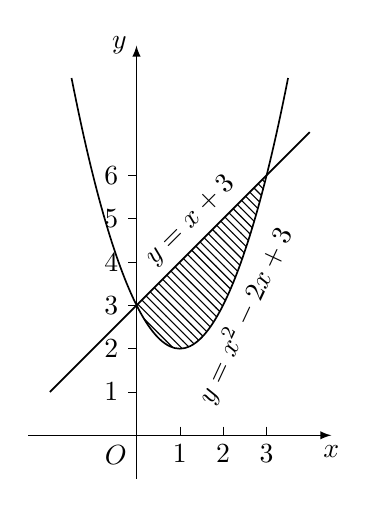
\begin{tikzpicture}[>=latex,scale=0.55]
  \draw[->](-2.5,0)--(4.5,0)node[below]{$x$};
  \draw[->](0,-1)--(0,9)node[left]{$y$};
  \node at (0,0)[below left]{$O$};
  \draw[semithick](-1.5,8.25)parabola bend(1,2)(3.5,8.25);
  \draw[semithick](-2,1)--(4,7)node[pos=0.6,sloped,above]{$y=x+3$};
  \foreach \x in {1,2,3}
    { \draw[very thin](\x,0.2)--(\x,0)node[below]{$\x$}; }
  \foreach \x in {1,...,6}
    { \draw[very thin](0,\x)--(-0.2,\x)node[left]{$\x$}; }
  \fill[pattern=north west lines](0,3)parabola bend(1,2)(3,6);
  \node at (2,3)[rotate=65,below]{$y=x^2-2x+3$};
\end{tikzpicture}
\end{document}